\documentclass{article} % For LaTeX2e
\usepackage{nips15submit_e,times}
\usepackage{hyperref}
\usepackage{graphicx}
\usepackage{amsmath}
\usepackage{amsthm}
\usepackage{graphicx}
\usepackage{caption}
\usepackage{subcaption}
\usepackage{lmodern}
\usepackage{titlesec}
\usepackage{longtable}
\usepackage{geometry}
\usepackage{multirow}
\usepackage{listings}
\usepackage{amsfonts}
\usepackage{algorithm}
\usepackage{algpseudocode}
\usepackage{multirow}
\usepackage{array}
\usepackage{url}

\author{
Thomas Nedelec \\
MSc Machine Learning\\
\texttt{thomas.nedelec.15@ucl.ac.uk} \\
\And
Michal Daniluk \\
MSc Machine Learning\\
\texttt{michal.daniluk.15@ucl.ac.uk} \\
}
\title{Supervized Learning: Assignment 1}




\newcommand{\fix}{\marginpar{FIX}}
\newcommand{\new}{\marginpar{NEW}}

\nipsfinalcopy % Uncomment for camera-ready version

\begin{document}


\maketitle

\section{Exercise 1: Least Square Regression: effect of the training set size}
We generated a noisy random data set, containing 600 samples, as $y_i = x_i'w + n_i$, where each $x_i$ and $n_i$ are drawn from the standard normal distribution. We splitted the data into a training set of size 100 a test set of size 500. We compute the mean squared error on both the training and test sets. Figure \ref{fig:lsr} shows examples of different training sets and estimated regression $w$.

 \begin{figure}[h]
\center
\begin{tabular}{ccc}
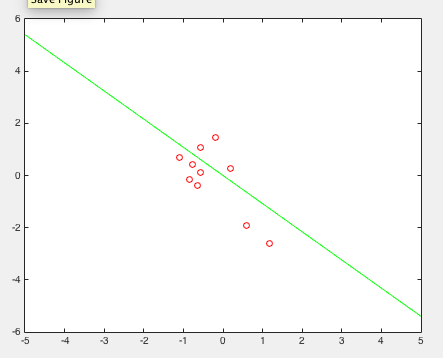
\includegraphics[width=0.3\textwidth]{10points}&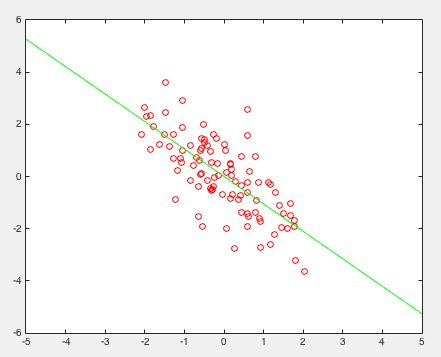
\includegraphics[width=0.3\textwidth]{100points}&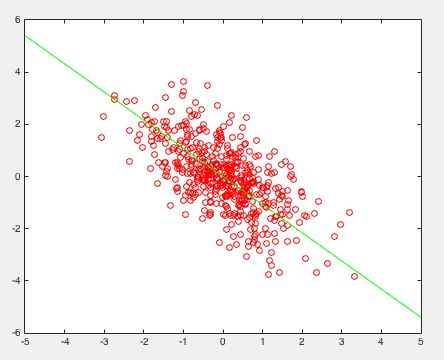
\includegraphics[width=0.3\textwidth]{500points}
\end{tabular}
\caption{ (a) training set of 10 points (b) training set of 100 points (c) the entire data set}
\label {fig:lsr}
\end{figure} 

Figure \ref{fig:resultMatrix1} illustrates the ''2 x 2'' table of averages mean square error for both training and test sets, on both 10 and 100 element-size training set.
\begin{figure}[h]
\begin{center}
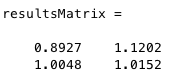
\includegraphics[width=0.4\textwidth]{resultsMatrix}
\end{center}
\caption{Average mean square error for both training and test sets, on both 10 and 100 element-size training set.}
\label{fig:resultMatrix1}
\end{figure}

We can observe that increasing the size of training set lets to decrease the average mean error on the test set. It's because, the larger training set prevents us from overfitting our model and give us a better overview of data. 
However, it increased the average mean error on train set.
With increasing the size of training set, the average error on the test and train set became similar. The average error on test set is larger than on train set. It is clear, because we have seen the train data before and haven't seen the test data.

\section{Exercise 2: Least Square Regression: effect of dimensionality}
We repeated the task in exercise 1, but with 10-dimensional data sets. Figure \ref{fig:resultMatrix2} illustrates the ''2 x 2'' table of averages mean square error for both training and test sets, on both 10 and 100 element-size training set.
\begin{figure}[h]
\begin{center}
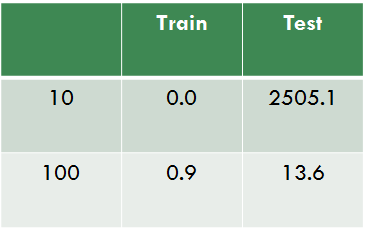
\includegraphics[width=0.4\textwidth]{resultsMatrix2}
\end{center}
\caption{Average mean square error for 10-dimensional data for both training and test sets, on both 10 and 100 element-size training set.}
\label{fig:resultMatrix2}
\end{figure}

For 10-sample training set, we obtain the average mean square error $0$ for train set and $2505.1$ for test set. We have 10-dimensional data and 10 samples, so we can accurately predict $y_i$ without any errors. However, the prediction is overfitted to the training data and we have a large error for test set. Increasing number of samples to 100 helps to decrease average error on test set. Average error for train set is bigger than for 10 samples, but our goal is to decrease test error.

\section{Ridge regression}

The regularization is a way to reduce the freedom of the classifier in order to improve the generalization and reach a better test set average error. 
\\ To implement ridge regression, we would like to minimize according to \textit{w} the cost function, 
\begin{equation}
\gamma w^{T}w + \frac{1}{l} \sum_{i=1}^{l}(x_{i}^{T}w - y_{i})^{2}.
\end{equation}
Using the notation $X=(x_{1}, x_{2},...,x_{l})^{T}$, a matrix containing the training sample vectors as its rows, we can rewrite the cost function as: 
\begin{equation}
\gamma w^{T} w + \frac{1}{l} Tr((Xw - Y)^{T}(Xw - Y))
\end{equation}
Taking derivative according to w, we reach: 
\begin{equation}
2\gamma w + 2 \frac{1}{l} (X^{T}Xw - 2Y^{T}X)=0
\end{equation}
To reach the conditions for optimality, we set the previous equation to zero and we reach: 
\begin{equation}
w=(\gamma l Id +X^{T}X)^{-1}Y^{T}X
\end{equation}
because if $\gamma*l \ne 0$ $(\gamma l Id +X^{T}X)$ is non-singular.

$\gamma l Id +X^{T}X $ is symetric.

We consider $u \in \mathbb{R}^{d}$:
\begin{align*}
\langle (\gamma l Id +X^{T}X)u,u \rangle &= \langle \gamma l u,u \rangle + \langle X^{T}X,u \rangle
\\  &= \gamma l \langle  u,u \rangle + \langle X u, X u \rangle
\\ &= \gamma l ||u||^{2} + ||Xu||^{2} > 0 \textit{ for u $\ne$ 0}
\end{align*}
Thus $\gamma l Id +X^{T}X$ is definite positve. 

\section{Effect of the regularisation parameter}

First, the graph \ref{fig:ex4_100} shows that if gamma is too high, the training error and test error increase dramatically. It is intuitive because when gamma is high the algorithm is far more likely to minimize $||w||$  rather than the training error.

 \begin{figure}[h]
\center
 \begin{subfigure}[b]{0.45\textwidth}
        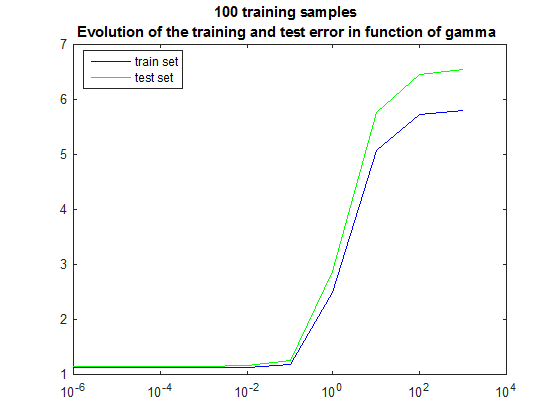
\includegraphics[width=\textwidth]{4_100}
        \caption{One run.}
    \end{subfigure}
    \begin{subfigure}[b]{0.45\textwidth}
        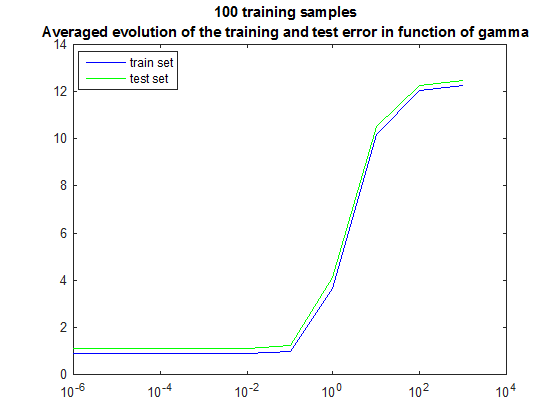
\includegraphics[width=\textwidth]{4_100_avg}
        \caption{Averaged on 200 runs.}
    \end{subfigure}
    \caption{Evaluation of the training error and test error in function of gamma for 100 training samples.}
    \label{fig:ex4_100}
\end{figure}

We have an optimal point corresponding to inflection point of the curve in order to select $\gamma$. Nevertheless, the training set error is not a sufficiently good guidance to select the regularization parameter because the charts are quite different. 

However, when we average the training error on 200 runs, we can observe that now the test error and the training error are now almost identical.

A way to select the optimal $\gamma$ would be to plot the error on the training set averaged on a certain number of runs of the algorithm and select the optimal $\gamma$ on this curve. 


 \begin{figure}[h]
\center
 \begin{subfigure}[b]{0.45\textwidth}
        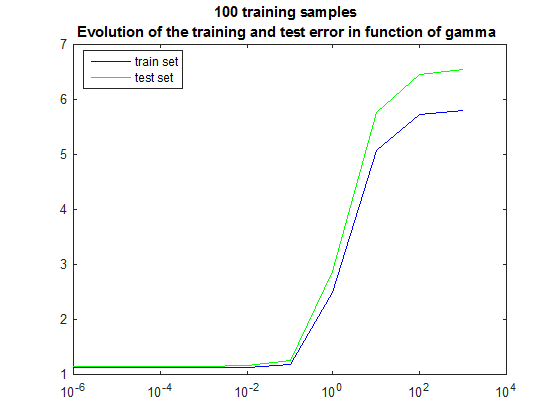
\includegraphics[width=\textwidth]{4_100}
        \caption{One run.}
    \end{subfigure}
    \begin{subfigure}[b]{0.45\textwidth}
        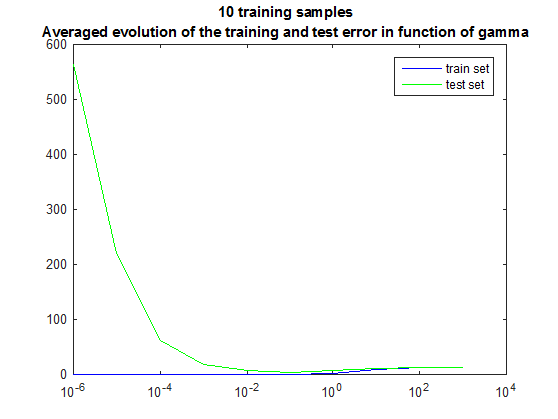
\includegraphics[width=\textwidth]{4_10_avg}
        \caption{Averaged on 200 runs.}
    \end{subfigure}
    \caption{Evaluation of the training error and test error in function of gamma for 10 training samples.}
    \label{fig:ex4_10}
\end{figure}

Figure \ref{fig:ex4_10} shows ..............


\section{Tuning the regularization parameter using a validation set}
 \begin{figure}[h]
\center
 \begin{subfigure}[b]{0.45\textwidth}
        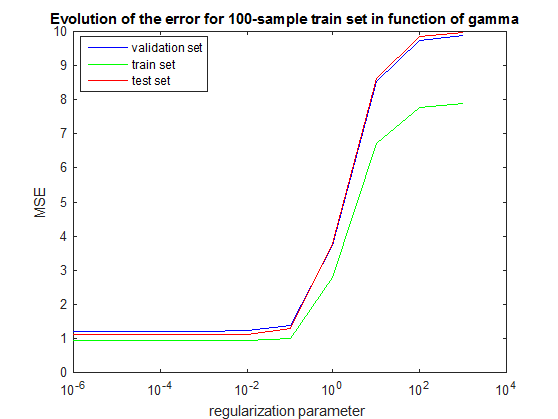
\includegraphics[width=\textwidth]{5_100}
        \caption{XXX}
    \end{subfigure}
    \begin{subfigure}[b]{0.45\textwidth}
        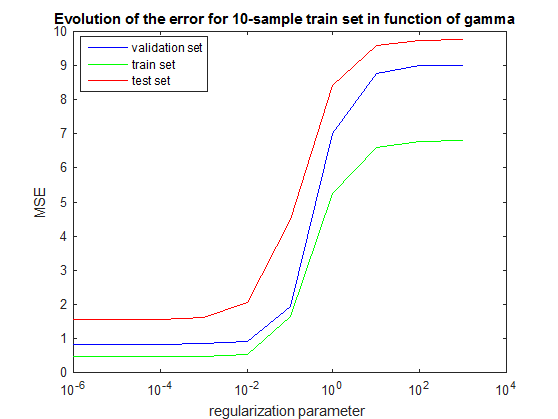
\includegraphics[width=\textwidth]{5_10}
        \caption{XXX}
    \end{subfigure}
    \caption{XXXX.}
    \label{fig:ex5}
\end{figure}


\section{Tuning the regularization parameter using cross validation}
We use 5-fold cross validation to tune the regularization parameter. Figure \ref{fig:ex6} shows cross-validation score on top of the training and test set error for different values $\gamma = \{10^{-6}, 10^{-5}, \dots, 10^3 \}$ of the regularization parameter.

\begin{figure}[h]
    \centering
    \begin{subfigure}[b]{0.45\textwidth}
        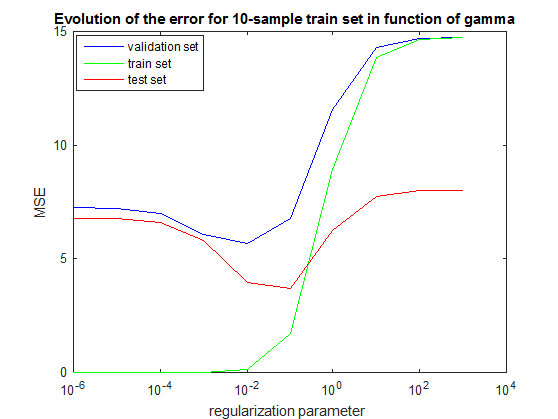
\includegraphics[width=\textwidth]{ex6_10}
        \caption{10-sample training set}
    \end{subfigure}
    \begin{subfigure}[b]{0.45\textwidth}
        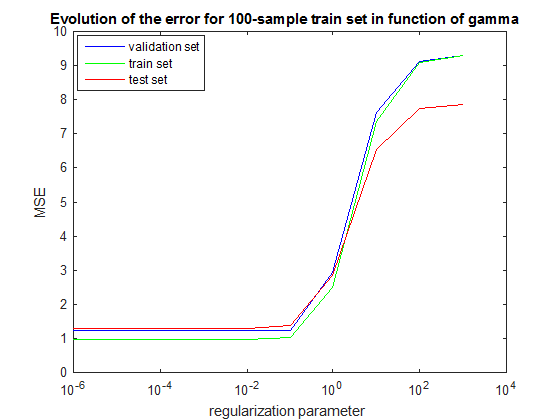
\includegraphics[width=\textwidth]{ex6_100}
        \caption{100-sample training set}
    \end{subfigure}
    \caption{Evaluation of the mean square error in function of gamma for different number of training examples.}
    \label{fig:ex6}
\end{figure}

Cross validation error is a good estimation of error for test set for both 10 and 100 samples. 


\section{Comparison of  $\gamma$ tuning methods}
The goal of this exercise is to generate 200 such data as in above exercises and tune the regularization parameter $\gamma$ using three methods. The results of average test error and standard deviation of the errors for 10 sample set-up are presented below:

\begin{enumerate}
\item By minimizing the training error
\begin{itemize}
\item Test set error: $163.9892$
\item Standard deviation of error: $508.3517$
\end{itemize}
\item By minimizing the validation error (80\% / 20 \% split)
\begin{itemize}
\item Test set error: $35.5974$
\item Standard deviation of error: $192.3498$
\end{itemize}
\item By minimizing the 5-fold cross validation error
\begin{itemize}
\item Test set error: $6.2890$
\item Standard deviation of error: $10.1677$
\end{itemize}
\end{enumerate}

The best results gives tunning regularization by minimizing the 5-fold cross validation error. Our model has only 10 samples and it's very prone to overfitting, so tunning the regularization parameter is very important in this case. Minimizing the 5-fold cross validation error gives us reasonable results despite the fact that training set is very small. Minimizing the training error doesn't seem to be a good approach, because the test set error and  standard deviation of error are very big. Using only one validation set gives us better results but still not such good as using cross validation method.


The results of average test error and standard deviation of the errors for 100 sample set-up are presented below:

\begin{enumerate}
\item By minimizing the training error
\begin{itemize}
\item Test set error: $1.1202$
\item Standard deviation of error: $0.0831$
\end{itemize}
\item By minimizing the validation error (80\% / 20 \% split)
\begin{itemize}
\item Test set error: $ 1.1529$
\item Standard deviation of error: $ 0.1283$
\end{itemize}
\item By minimizing the 5-fold cross validation error
\begin{itemize}
\item Test set error: $1.1208$
\item Standard deviation of error: $0.0848$
\end{itemize}
\end{enumerate}
First of all, the results are much better than for 10 sample set-up, but is is because we increase training set. Secondly,  differences between results for each method are very small. It's because, we have a big enough train set and regularization isn't really necessary. The model isn't prone to overfitting. 

\section{Kernel Ridge Regression}
In this exercise we will perform kernel ridge regression on the Boston data set with the Gaussian kernel, which is defined as:
\begin{equation}
K(x_i,x_j) = exp(-\frac{|| x_i - x_j||^2}{2 \sigma^2})
\end{equation}

We created a function \textit{kridgereg.m} to perform kernel ridge regression using equation $\alpha^* = (K + \gamma l I_l)^{-1}y$. We don't explicitly use a matrix inverse instead use the matrix left division operator. According to the Matlab documentation, \textit{mldivide} is a more efficient way to solve a linear equation $Ax = b$. If the solution does not exist or if it is not unique, the  \textit{mldivide} operator issues a warning.

Then, we created a function called \textit{dualcost.m} to calculate the Mean Squared Error (MSE) using equation:
\begin{equation}
mse = \frac{1}{l}(K_{test} \alpha - y)'(K_{test} \alpha - y)
\end{equation}

We perform kernel ridge regression on the training set using five-fold cross-validation with different values of $\gamma$ and $\sigma$. Figure \ref{fig:ex910} shows the cross-validation error as a function of $\gamma$ and $\sigma$. 
\begin{figure}[h]
    \centering
    \begin{subfigure}[b]{0.45\textwidth}
        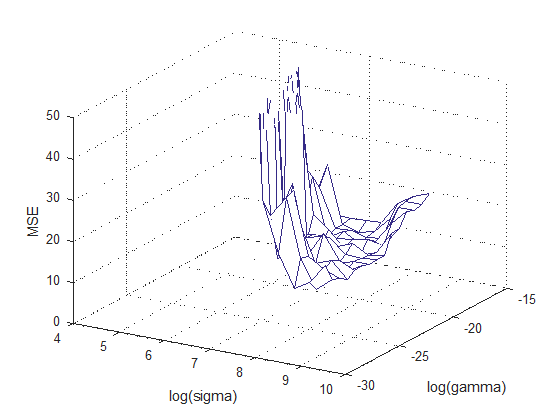
\includegraphics[width=\textwidth]{ex910_1}
    \end{subfigure}
    \begin{subfigure}[b]{0.45\textwidth}
        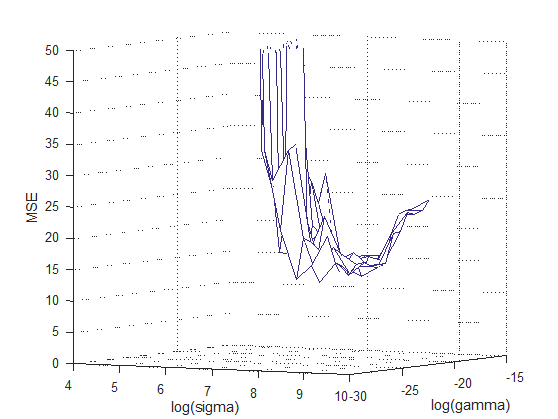
\includegraphics[width=\textwidth]{ex910_2}
    \end{subfigure}
    \caption{Cross-validation error as a function of $\gamma$ and $\sigma$.}
    \label{fig:ex910}
\end{figure}
The best results are for values $\gamma = 2^{-31}$ and $\sigma = 2^{12}$. The MSE on the training data $= 8.8392$ and on the test set $= 13.8215$.

Then, we repeat those steps over 20 random splits of data. Our results for exercise 9 and 10 are summarized in the table:
\begin{center}
\begin{tabular}{|  l c r|}
  \hline
  \textbf{Method} & \textbf{MSE train} & \textbf{MSE test} \\
  Naive Regression & 84.5706 $ \pm $ 3.7489 & 84.3933 $ \pm $ 7.3810\\
 Linear Regression (attribute 1) & 71.9206 $ \pm $ 3.7157& 71.7623$ \pm $ 7.2524\\
  Linear Regression (attribute 2) & 73.4863 $ \pm $ 4.2998& 73.7122$ \pm $ 8.4777\\
 Linear Regression (attribute 3) & 64.8467 $ \pm $ 4.6972& 64.7529$ \pm $ 9.1959\\
 Linear Regression (attribute 4) & 81.3032 $ \pm $ 3.2466& 83.5478$ \pm $ 6.3118 \\
 Linear Regression (attribute 5) & 69.1346 $ \pm $ 3.6979& 69.0250$ \pm $ 7.8448\\
 Linear Regression (attribute 6) & 43.0045 $ \pm $ 4.6585& 45.4416$ \pm $ 9.3804\\
 Linear Regression (attribute 7) & 72.6169 $ \pm $ 4.3741& 72.4109$ \pm $ 8.5975\\
 Linear Regression (attribute 8) & 79.1138 $ \pm $ 4.3852& 79.6780$ \pm $ 8.5893\\
 Linear Regression (attribute 9) & 72.4303 $ \pm $ 4.2039& 71.9495$ \pm $ 8.2573\\
 Linear Regression (attribute 10) & 66.3728 $ \pm $ 4.5274& 65.3491$ \pm $ 8.9139\\
 Linear Regression (attribute 11) & 63.3372 $ \pm $ 3.9821& 61.7821$ \pm $ 7.9450\\
 Linear Regression (attribute 12) & 75.1591 $ \pm $ 3.8102& 75.1225$ \pm $ 7.5406\\
  Linear Regression (attribute 13) & 38.2716 $ \pm $ 2.1729& 39.1051$ \pm $ 4.2303\\
  Linear Regression (all attributes) & 23.1232 $ \pm $ 2.9711& 27.8889$ \pm $ 6.2950\\
 Kernel Ridge Regression  & 7.9308$ \pm $1.3363 & 13.7928$ \pm$ 2.4398\\
  \hline
\end{tabular}
\end{center}

\section*{Part 2}
\subsection*{1}

\end{document}
